%% Isolon --- EuroSys 2027 Fall (anonymous SIGPLAN draft)
%% Public living paper uses a different title and system name (CFP §concurrent).
%% Do not put author names, affiliations, URLs, or unique product markers here.
\documentclass[sigplan,10pt,anonymous,review]{acmart}

\setcopyright{none}
\settopmatter{printfolios=true,printccs=true,printacmref=true}
\renewcommand\footnotetextcopyrightpermission[1]{}
\pagestyle{plain}

\acmConference[EuroSys '27]{European Conference on Computer Systems}{April 19--24, 2027}{Morocco}
\acmYear{2027}
\acmISBN{}
\acmDOI{}

\usepackage{booktabs}
\usepackage{graphicx}
\usepackage{tikz}
\usetikzlibrary{arrows.meta,positioning,fit,calc}

%% Grayscale-safe tables (CFP: figures readable without color).
\acmSubmissionID{eurosys27-fall-anon}

\begin{document}

\title[Exclusive Guest-Physical Isolation]{Exclusive Guest-Physical Isolation in a Type-1 Hypervisor: A Machine-Checked Ghost Model and a Bare-Metal Runtime}

\begin{abstract}
Type-1 hypervisors isolate guest memory with extended page tables, yet
production stacks treat that isolation as a testing problem. This paper
reports Isolon, a clean-slate Type-1 hypervisor that boots as a single UEFI
binary on production two-socket Xeon servers and is designed so the
security-critical path can be machine-checked.

Isolon confines formal proofs to a Proven Core. The headline property is
\emph{exclusive ownership} of host frames: every valid guest-physical to
host-physical mapping is owned by exactly one guest and belongs to neither
the hypervisor nor any other guest. We discharge that property in a
host-only Verus ghost model through map, unmap, EPT-violation handling, and
a page-transfer primitive---80 lemmas verified, 0 errors, with no
\texttt{admit} on the exclusivity path---under a frozen SMT toolchain pin.
Live executable EPT remains at spec-written maturity: a runtime ownership
registry plus assertions, not a bisimulation of the EFI. Device emulation,
the management plane, and guest firmware are outside the Proven Core and
are not claimed as theorems.

On a real PowerEdge R640 we reproduce VMX bring-up, EPT identity mapping, an
unmodified Linux shell, multi-VM probes, durable host-NIC HTTP, and
guest-firmware CD-ROM boot. Nested VT-x completed a Linux distro
install-to-disk; nested virtualization is not that server. We report those
facts, name the ghost/executable gap, and stop there.
\end{abstract}

\begin{CCSXML}
<ccs2012>
 <concept>
  <concept_id>10011007.10011074.10011099.10011102</concept_id>
  <concept_id>10002978.10011006.10011050</concept_id>
  <concept_id>10011007.10011006.10011008.10011009.10011015</concept_id>
  <concept_desc>Software and its engineering~Software verification</concept_desc>
  <concept_desc>Security and privacy~Logic and verification</concept_desc>
  <concept_desc>Software and its engineering~Virtual machines</concept_desc>
  <concept_significance>500</concept_significance>
 </concept>
</ccs2012>
\end{CCSXML}

\ccsdesc[500]{Software and its engineering~Software verification}
\ccsdesc[500]{Software and its engineering~Virtual machines}
\ccsdesc[300]{Security and privacy~Logic and verification}

\keywords{formal verification, Type-1 hypervisor, EPT, Verus, exclusive ownership}

\maketitle

\section{Introduction}

A hypervisor's job is to make one computer look like several, without letting
those several computers look at each other. On modern Intel servers the
mechanism that actually enforces that is Extended Page Tables
(EPT)~\cite{intel-sdm}. If EPT is wrong, two guests share a frame, or a
guest sees hypervisor memory, and no amount of management-API polish repairs
it.

Commercial Type-1 stacks---ESXi, Xen~\cite{barham2003xen},
KVM~\cite{kivity2007kvm}---are large, mature, and tested. They are not
accompanied by a machine-checked isolation theorem for the frames they hand
to guests. Research systems that \emph{are} proved
(seL4~\cite{klein2009sel4,klein2014comprehensive},
CertiKOS~\cite{gu2016certikos}, Komodo~\cite{ferraiuolo2017komodo}) target
microkernels, certified kernels, or enclaves. They are not a single UEFI
binary aimed at the PowerEdge fleet already in the rack.

Isolon takes a narrower bet. It is a clean-slate Type-1 hypervisor written in
Rust. It compiles to one \texttt{.efi}. It boots on hardware we own and can
serial-log: Dell PowerEdge R640-class machines. Formal verification is an
architectural constraint, not a post-hoc whitepaper. We picked
Verus~\cite{lattuada2023verus,lattuada2024verus} for SMT proofs of ghost
state and Kani~\cite{vanhattum2022kani} for bounded checking of
\texttt{unsafe}, and we defined a four-level maturity ladder so the project
can ship at runtime-enforced or spec-written maturity when a full proof is
still in flight.

The headline theorem is exclusive ownership of host frames. We prove it of a
\emph{ghost model}, not of the EFI that leaves the compiler. That distinction
is the paper. Claiming ``the hypervisor is proved'' would be proving the
wrong thing~\cite{klein2014comprehensive}: a convenient proxy. We discharge 80
Verus lemmas with 0 errors; live executable EPT is a 705-line ownership
registry with contracts and assertions. Device emulation, HTTP, the SPA,
ISO handling, and guest firmware are outside the Proven Core.

This paper makes three contributions:

\begin{enumerate}
\item \textbf{A tight isolation theorem and a discharged ghost model.}
  Exclusive ownership is four conjuncts over two ghost maps (frame
  $\rightarrow$ guest, and $(\mathrm{guest},\mathrm{GPA})\rightarrow$ frame).
  Named theorems cover 4K map/unmap (one guest and $N$ guests), scoped
  ghost$\leftrightarrow$executable refinement, 2M/1G spans, NUMA affinity,
  hardware 2M-leaf decode, EPT-violation dispositions, and a page-transfer
  primitive. Under a frozen Verus pin the crate reports 80 verified, 0
  errors, with no \texttt{admit} on that path.

\item \textbf{An architecture that keeps the proved surface small} while
  still shipping a UEFI Type-1 hypervisor: a 15{,}000-line Proven Core
  budget, a host-only proof crate that is deliberately not linked into the
  \texttt{.efi}, and an explicit refusal to mutate third-party firmware
  internals to manufacture forward progress.

\item \textbf{A split evaluation.} Lab/CI hosts hold L3. A real PowerEdge
  R640 holds L1 runtime through Linux shell, multi-VM probes, host-NIC
  HTTP, and guest-firmware El Torito. Nested VT-x completed a distro
  sysinstall. We do not collapse those three columns into one claim.
\end{enumerate}

Isolon is not seL4 for hypervisors and is not a verified KVM. It is a
small exclusive-ownership model that we actually discharge, sitting next to
a hypervisor we actually boot on iron, with the gap named in the same
breath.

\section{Threat Model and Non-Goals}

\subsection{Why memory isolation is the headline}

A Type-1 hypervisor is the TCB for every guest it runs. CPUID and MSR
firewalls, interrupt injection, and the hypercall door all matter. None of
them matter if EPT can map the same host frame to two guests, or to a guest
and the hypervisor, without anyone noticing. We therefore name
\emph{exclusive ownership of host frames} as the property we prove, not
``the guest seemed isolated in tests.''

\subsection{In scope}

We assume:

\begin{itemize}
\item A \textbf{malicious or compromised guest} (ring-0 Linux, firmware, or
  installer) that may issue any architected VM exit: EPT violation, CPUID,
  MSR, I/O, hypercall, HLT, exception.
\item \textbf{Buggy device emulation} outside the Proven Core (virtio, IDE/ATAPI,
  UART). Bugs there can DoS a guest or confuse an installer; they must not
  become a second EPT mapping of a Proven Core frame.
\item \textbf{Operator error} (wrong ISO, exhausted USB stick). Audit events
  record what happened; they do not enlarge the theorem.
\end{itemize}

We do \emph{not} assume a correct third-party guest firmware. Forcing a
foreign firmware's WaitForEvent internals to skip a check produced a
NULL-event page fault and a dead loop. Product ISO boot now uses firmware we
author. That firmware is \textbf{outside} the Proven Core.

\subsection{Out of scope for the theorems}

\begin{itemize}
\item The Intel SDM's VMX/EPT hardware behaves as documented~\cite{intel-sdm}.
\item The frozen Verus/SMT stack is trusted for the ghost proofs.
\item Host physical memory given to the allocator is the memory the
  machine has.
\item DMA from devices we do not model (untrusted NICs, USB) is a future
  confinement problem, not a discharged lemma.
\item Nested VT-x on a lab server is not a proof about a PowerEdge R640.
\item Full x86 ISA / VMCS host-state correctness is inside the Proven Core
  \emph{budget} and is not at proof-complete maturity beside the EPT crate.
\end{itemize}

\section{Isolon Architecture}

\subsection{Single binary}

Everything compiles to one UEFI PE/COFF image. Kernel, initrd, Web UI, and
schemas are compressed sections, decompressed on first use. The size target
is 15~MB with a 20~MB hard limit. There is no host Linux, no package
manager, and no config tree the operator must get right before the first
serial line.

\subsection{Proven Core boundary}

Only the modules in Table~\ref{tab:core} are in scope for Verus
specifications and progressive proofs. Everything else uses Rust's type
system, testing, and review. Promotion into the Proven Core requires a
written architecture decision; the default answer is no. The hard cap is
15{,}000 lines including proof scaffolding.

\begin{table}[t]
  \caption{Proven Core budget (cap, not an L3 claim per row).}
  \label{tab:core}
    \begin{tabular}{lrp{3.4cm}}
    \toprule
    Module & Est.\ LOC & Why inside \\
    \midrule
    VMX lifecycle & 800 & VMXON/VMXOFF leave CPU mode \\
    VMCS management & 1{,}500 & Host-state corruption \\
    EPT engine & 2{,}000 & Isolation mechanism \\
    Frame allocator & 1{,}500 & Double-alloc / UAF \\
    vCPU state & 1{,}000 & Save/restore leaks \\
    Interrupt injection & 800 & Guest privilege \\
    Hypercall door & 500 & Only intentional channel \\
    MSR/CPUID/CR firewalls & 1{,}200 & Host feature subversion \\
    Audit-log integrity & 600 & Tamper-evident trail \\
    IPI confinement & 500 & Cross-VM IPI \\
    \midrule
    Cap (code + scaffolding) & 15{,}000 & --- \\
    \bottomrule
  \end{tabular}
\end{table}

Lived split, as of this submission: the machine-checked exclusivity theorems
live in a host-only crate (\texttt{ept\_model}, 2{,}366 lines) that is
\emph{not} linked into the \texttt{.efi}. The executable EPT ownership
registry is 705 lines at spec-written maturity. Device emulation, HTTP, the
SPA, ISO, guest firmware, iDRAC, and migration tooling are outside.

\subsection{Hardware}

Dell PowerEdge R640 / R650 / R660. Low-risk, self-sufficient surfaces (serial
via iDRAC virtual console, SMBIOS/ACPI topology, onboard LOM) are in
scope. OEM RAID health schemas are not a blocker for the theorems or for
the single-host product loop.

Code in the Proven Core is required to document invariants at the function
boundary, keep \texttt{unsafe} blocks minimal, and tag each of them for
bounded checking. Mutable globals require a lock and a justification
comment. We use explicit state machines rather than boolean flags. These
rules are how a codebase stays L3-shaped when most modules are still L1:
the later proof should not require a rewrite of ownership.

\subsection{Maturity ladder}

We use four levels, kept even after a proof lands (runtime asserts stay):

\begin{itemize}
\item \textbf{L0} documented invariants in comments.
\item \textbf{L1} runtime \texttt{assert!}/\texttt{debug\_assert!} plus Kani
  on \texttt{unsafe}.
\item \textbf{L2} Verus specifications with ghost state and contracts.
\item \textbf{L3} \texttt{cargo verus verify} succeeds for the claimed
  surface.
\end{itemize}

Fallback is Verus $\rightarrow$ Kani $\rightarrow$ asserts and fuzz. The
architecture always aims at L3; shipping is allowed at L1/L2 when L3 is
still open, provided the paper does not upgrade the label.

Proven Core modules follow a four-file layout: executable Rust, a spec
file, a proof file, and tests (Kani + unit). The exclusivity theorems of
record do not use that layout. They live in one \texttt{verus!} block in
\texttt{ept\_model/src/lib.rs}, verified with \texttt{cargo verus verify -p
ept\_model}. Putting them beside live \texttt{memory/ept.rs} would imply
the EFI crate is L3. It is not.

\section{Exclusive Ownership}

\subsection{Statement}

\begin{quote}
For every valid EPT mapping from a guest-physical address to a host-physical
frame, that frame is exclusively owned by the mapping guest and belongs to
neither the hypervisor nor any other guest.
\end{quote}

``Exclusively owned'' means exactly one guest holds a mapping to that frame
at any moment. ``Belongs to neither'' means the frame is absent from the
hypervisor's page tables and from every other guest's EPT. The property
must hold across map, unmap, EPT-violation handling, and live-migration page
transfer.

\subsection{Ghost state}

The ghost model is two finite maps (Figure~\ref{fig:maps}):

\begin{itemize}
\item $\mathit{owned}: \mathit{FrameId} \rightharpoonup \mathit{GuestId}$
\item $\mathit{by\_gpa}: (\mathit{GuestId} \times \mathit{Gpa}) \rightharpoonup \mathit{FrameId}$
\end{itemize}

Guest id $0$ is reserved (hypervisor / unmapped). 4K steps require
page-aligned GPAs. A map step is enabled only when the frame is free and the
$(\mathrm{guest},\mathrm{GPA})$ pair is free. An unmap step is enabled only
when that pair is present.

\begin{figure}[t]
\centering
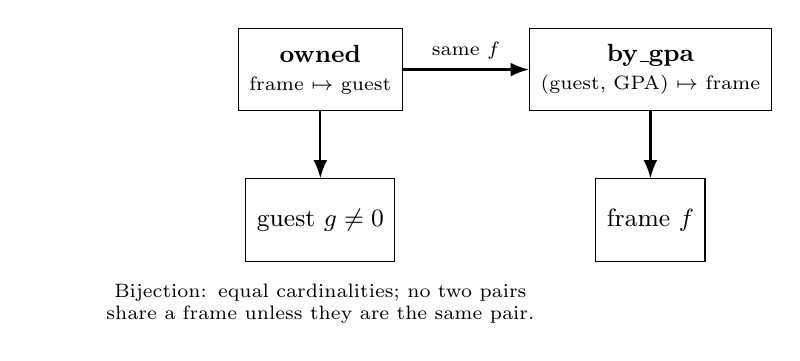
\begin{tikzpicture}[
  font=\small,
  box/.style={draw,align=center,inner sep=4pt,minimum height=1.05cm},
  arr/.style={-{Latex},thick}
]
\node[box] (owned) {\textbf{owned}\\[-1pt]{\scriptsize frame $\mapsto$ guest}};
\node[box,right=1.6cm of owned] (bygpa) {\textbf{by\_gpa}\\[-1pt]{\scriptsize (guest, GPA) $\mapsto$ frame}};
\node[box,below=0.85cm of owned] (guest) {guest $g\neq 0$};
\node[box,below=0.85cm of bygpa] (frame) {frame $f$};
\draw[arr] (owned) -- (guest);
\draw[arr] (bygpa) -- (frame);
\draw[arr] (owned.east) -- node[above,font=\scriptsize]{same $f$} (bygpa.west);
\node[below=0.15cm of guest, font=\scriptsize, text width=7.2cm, align=center]
  {Bijection: equal cardinalities; no two pairs share a frame unless they are the same pair.};
\end{tikzpicture}
\caption{Ghost EPT ownership registry. Exclusive ownership is four
conjuncts: every owned frame has a matching \texttt{by\_gpa} witness; every
\texttt{by\_gpa} entry has a matching owner; a frame is the image of at most
one pair; the two maps have equal length.}
\Description{Two boxes labeled owned and by\_gpa, with arrows to a guest and a frame, noting a bijection between the maps.}
\label{fig:maps}
\end{figure}

The predicate (verbatim from the crate, names only) is:

\begin{verbatim}
exclusive_ownership(m)  iff
  forall f.  owned.contains(f)
    ==> exists g,a. by_gpa[(g,a)] = f
                 /\ owned[f] = g
  /\ forall g,a. by_gpa.contains((g,a))
    ==> owned.contains(by_gpa[(g,a)])
        /\ owned[by_gpa[(g,a)]] = g
  /\ forall g1,a1,g2,a2.
       by_gpa[(g1,a1)] = by_gpa[(g2,a2)]
         ==> g1=g2 /\ a1=a2
  /\ owned.len() = by_gpa.len()
\end{verbatim}

Empty maps satisfy it. A hypervisor frame is modelled as \emph{not} being
in $\mathit{owned}$: the ghost registry only tracks guest-held frames. That
is the ``belongs to neither'' half, as a modelling choice---the EFI's own
page tables are not in this crate.

\subsection{Steps}

A 4K step is $\mathsf{Map}\{g,a,f\}$ or $\mathsf{Unmap}\{g,a\}$. Enabled
steps preserve exclusive ownership (one-step lemma). Any finite sequence of
enabled steps preserves it (the historical single-guest theorem, whose
statement already allows distinct guest ids across steps; a second theorem
is named so CI can assert the $N$-guest post). A two-guest lemma maps two
distinct non-zero guests onto distinct free frames.

Large pages are spans of 4K frames (512 for 2M, $2^{18}$ for 1G). Span
map/unmap lemmas lift exclusivity to 2M/1G; unit lemmas record that 4K is a
one-frame span. NUMA lemmas couple a ghost SRAT/SLIT topology with
map/unmap so a mapped frame is recorded on its node. Hardware 2M-leaf
decode lemmas relate a leaf PTE encoding to an identity-map intent. None of
these lemmas are a full multi-level EPT walk of the EFI.

\subsection{EPT-violation dispositions}

An EPT miss is modelled as one of three dispositions:

\begin{itemize}
\item $\mathsf{EmulateNoMap}$ --- emulate MMIO (APIC / virtio) without
  installing a mapping. Registry unchanged.
\item $\mathsf{Reject}$ --- fail closed. Registry unchanged.
\item $\mathsf{ClaimMap}\{g,a,f\}$ --- demand-fill a 4K map, enabled only
  when that map step would be enabled.
\end{itemize}

Every enabled disposition preserves exclusive ownership. Emulate-then-claim
is a derived post.

\subsection{Page transfer}

Live migration of a frame is unmap-at-source then map-the-same-HPA at
destination. The step is enabled when source holds the GPA, destination GPA
is free, and guests are distinct and non-zero. Posts: destination owns the
frame at the new GPA; the source mapping is gone; exclusivity holds. This is a
ghost primitive. It is not vCenter vMotion, not a multi-host protocol, and
not a proof that the product migrate engine is correct. That engine is
outside the Proven Core.

\subsection{Theorems of record}

Table~\ref{tab:theorems} lists the named theorems. Supporting lemmas
(empty-exclusive, map-already-owned-unchanged, span preservation, mock
bring-up facts) are in the same crate. CI counts 80 verified functions.

\subsection{Proof sketch: map preserves exclusivity}

We sketch the 4K map case; unmap is the inverse bookkeeping. Assume
$\mathit{exclusive\_ownership}(m)$, $g\neq 0$, $a$ 4K-aligned,
$f\notin\mathrm{dom}(\mathit{owned})$, and $(g,a)\notin\mathrm{dom}(\mathit{by\_gpa})$.
Let $m' = m.\mathsf{ghost\_map}(g,a,f)$.

\emph{Witness.} For the new frame $f$, the pair $(g,a)$ is the witness
required by conjunct~1. Old frames keep their old witnesses because we
did not delete \texttt{by\_gpa} entries.

\emph{Owner match.} The new \texttt{by\_gpa} entry points at $f$, and
$\mathit{owned}'[f]=g$. Old pairs are unchanged.

\emph{Uniqueness.} Suppose two pairs in $m'$ share a frame. If that frame
is $f$, both pairs must be $(g,a)$ because $f$ was free. If not, uniqueness
in $m$ applies.

\emph{Cardinalities.} Both maps gain one key, so lengths stay equal.

Verus discharges this with map lemmas from \texttt{vstd} (broadcast
\texttt{group\_map\_lemmas} / \texttt{group\_set\_lemmas}). The one-step
lemma case-splits on $\mathsf{Map}$ vs $\mathsf{Unmap}$. The sequence
theorem is induction on $\mathsf{Seq}$ length: the empty sequence is
trivial; the inductive step applies the one-step lemma and recurses.
The $N$-guest theorem is that same induction under a CI-facing name;
guest ids are already a field of each step.

\paragraph{What the SMT does not get for free.}
Span (2M/1G) map is not ``map 4K $k$ times'' as an opaque loop in
executable code. It is a ghost predicate that the 4K keys covering the
span are all free, then a bulk insert. The 2M lemma records that 512
aligned 4K frames constitute a 2M leaf; the 1G lemma records $2^{18}$.
Those facts are arithmetic lemmas, not a hardware page-walk.

Violation $\mathsf{ClaimMap}$ reuses the 4K map lemma. Emulate and reject
are identity on the registry; the proof is $m'=m$. Transfer is unmap then
map of the \emph{same} frame: after unmap, $f$ is free, so the destination
map is enabled. Posts are the destination owner and the absent source
key.

\paragraph{Modelling choice: hypervisor frames.}
Conjuncts quantify over \texttt{owned} and \texttt{by\_gpa}, not over the
EFI's own page tables. A hypervisor frame is exclusive in this model
because it is \emph{absent} from $\mathit{owned}$. That is the right
theorem for ``guests do not share guest frames.'' It is \emph{not} a
theorem that an executable bug cannot install a guest leaf pointing at
\texttt{.text}. Closing that would require the live EPT walker and the
HV page tables in the same proved artifact. They are not. Section~5 is
that sentence at L2.

\begin{table}[t]
  \caption{Named exclusivity theorems in the host-only crate.}
  \label{tab:theorems}
  \begin{tabular}{lp{4.6cm}}
    \toprule
    Theorem & Claim \\
    \midrule
    \texttt{single\_guest\_4k\_map\_unmap} & finite 4K sequences \\
    \texttt{n\_guest\_4k\_map\_unmap} & same discharge, $N$-guest name \\
    \texttt{concrete\_single/n\_guest\_refine} & scoped ghost$\leftrightarrow$exec \\
    \texttt{large\_page\_map\_unmap} & 2M/1G spans \\
    \texttt{numa\_map\_unmap\_affinity} & node affinity ghost \\
    \texttt{hw\_2m\_leaf\_refines\_identity} & 2M leaf encode \\
    \texttt{ept\_violation\_preserves} & miss dispositions \\
    \texttt{page\_transfer\_preserves} & unmap$\rightarrow$map handoff \\
    \texttt{alloc\_map\_unmap\_refines} & pool + EPT refine \\
    \bottomrule
  \end{tabular}
\end{table}

\section{The Ghost / Executable Gap}

A discharged ghost model is not a proved \texttt{.efi}. Isolon records that
as a first-class result, not a footnote.

Live EPT (\texttt{memory/ept.rs}, 705 lines) maintains an ownership registry
and asserts exclusive-ownership-shaped facts at map/unmap. Beside it sit
357 lines of spec/proof notes. Those notes are not the 80-lemma crate. The
host-only crate exists \emph{because} linking Verus into the UEFI target is
the wrong packaging: proofs run on a Linux CI host under a pinned Verus
release; the EFI is \texttt{x86\_64-unknown-uefi}.

Scoped refinement lemmas show that a concrete map representation, under a
restricted interpretation, commutes with ghost map/unmap for 4K (one
guest, then $N$ guests) and that an allocate-then-map path refines. They
are not a bisimulation of VMXON, VMCS host state, EPT pointer load, and
every MMIO emulator the EFI contains.

Consequences we accept in print:

\begin{itemize}
\item L3 is the ghost crate. Live EPT is L2.
\item VMX, VMCS, hypercalls, MSR firewalls, audit integrity, and IPI
  confinement are in the budget in Table~\ref{tab:core} and are not at L3
  beside \texttt{ept\_model}.
\item Iron serial logs raise confidence in the \emph{runtime path}. They do
  not raise Verus maturity. Lab L3 and R640 L1 are both real; they are not
  the same claim.
\end{itemize}

A prior self-review asked whether exclusive ownership is the property an
auditor cares about or a convenient proxy. The verdict was: in scope for
map/unmap/violation/transfer; ops gates (auth, PDF reports, HA, soak
metrics) correctly labelled outside. Independent third-party re-run of
\texttt{verus --verify} under the pin remains the auditor path. Bring-up
self-review is not a conference peer review.

\subsection{Live registry versus ghost maps}

The live engine is not a Verus \texttt{Map}. It is a bounded table:
\texttt{EptMap} holds at most 512 explicit 4K claims in production builds
(8 under Kani, so CBMC can unwind), plus a 16-slot range registry for the
precise identity window used at Linux bring-up. Map fails with
\texttt{AlreadyOwned} when a frame is taken. Invariants are checked with
\texttt{debug\_assert!} after mutating operations. A boot self-test maps a
bring-up guest, then asserts that a second guest cannot alias the same
frame.

That is the right shape for L1/L2. It is a different datatype from the
ghost model (finite maps of unbounded domain, no \texttt{MAP\_CAP}). The
scoped refine lemmas interpret a concrete map into ghost maps; they do
not prove that the 512-slot table implements those maps for every
reachable EFI state. If a 513th distinct 4K claim is required, the live
table saturates while the ghost theorem still holds of an abstract
\texttt{ghost\_map}. That mismatch is why we will not stamp L3 on
\texttt{memory/ept.rs} from the 80/0 line.

The range registry is another gap. Bring-up identity-maps a contiguous
window (hundreds of megabytes) without inserting hundreds of thousands of
4K ghost keys at runtime. The ghost large-page lemmas talk about spans;
the live precise window is a range claim plus hardware identity PTEs.
Correspondence is scoped (hardware 2M-leaf decode lemma + range
self-test), not ``every live PTE has a ghost key.''

\subsection{What would close the gap}

Three artifacts, none of which this paper claims:

\begin{enumerate}
\item A proved executable EPT walker whose leaves are in 1--1
  correspondence with \texttt{by\_gpa}, including the HV-vs-guest split
  (``belongs to neither'' as a fact about HV page tables, not as absence
  from a guest registry).
\item An IOMMU / DMA story: devices we do not model cannot write a
  guest-owned frame or a hypervisor frame.
\item Linking or replaying (1) on the UEFI target, or a refinement from
  the EFI binary's EPT root pointer to the ghost maps.
\end{enumerate}

Until then, ``memory isolation isn't tested; the ghost exclusivity
theorems are proved'' is the strongest true slogan. ``The hypervisor is
proved'' is false.

\section{Evaluation}

We evaluate three questions. (1)~Does the ghost model actually verify?
(2)~How large is the proved surface relative to the hypervisor?
(3)~What does the runtime do on a lab host versus a real R640?

\subsection{Proofs}

Toolchain: Verus \texttt{release/0.2026.07.12.0b42f4c} (content-addressed
Linux zip, SHA-256 pinned; CI never uses \texttt{latest}) and Kani 0.67.0.
The exclusivity crate is verified with \texttt{cargo verus verify -p
ept\_model}. The last closed host gate on that crate reported \textbf{80
verified, 0 errors}. No \texttt{admit} on the exclusivity path. We do not
invent a wall-clock for this PDF; the artifact is the crate plus the pin
(supplement).

Kani covers bounded \texttt{unsafe} in the live engine. That is L1 on
\texttt{unsafe}, not L3 on exclusive ownership.

\subsection{Size}

Table~\ref{tab:loc} is a line count on the tree used for this draft, not a
re-baseline of the 15{,}000-line cap. Ghost proofs of record are larger than
the live EPT engine. That is expected: the theorem lives in the crate we
can host-verify. The cap still applies to the Proven Core modules; most of
those rows are not at L3.

\begin{table}[t]
  \caption{Line counts (\texttt{wc -l}) for the EPT-related surface.}
  \label{tab:loc}
  \begin{tabular}{lrr}
    \toprule
    Path & Lines & Role \\
    \midrule
    \texttt{ept\_model/src/lib.rs} & 2{,}366 & L3 ghost + proofs \\
    \texttt{memory/ept.rs} & 705 & live EPT (L2) \\
    \texttt{ept\_spec.rs} + \texttt{ept\_proof.rs} & 357 & notes beside live \\
    frame allocator + spec & 362 & allocator + ghost set \\
    \bottomrule
  \end{tabular}
\end{table}

\subsection{Runtime: lab host versus R640}

Table~\ref{tab:split} is the split. Cells are contemporaneous serial or
host-test evidence, not a wish list. Nested VT-x is a third column because
operators (and reviewers) otherwise collapse it into iron.

\begin{table*}[t]
  \caption{Split evaluation. Nested VT-x $\neq$ PowerEdge. Host Verus $\neq$ EFI.}
  \label{tab:split}
  \small
  \begin{tabular}{lccc}
    \toprule
    Surface & Lab / CI host & Nested VT-x & PowerEdge R640 \\
    \midrule
    Verus exclusivity (80 / 0) & yes (L3) & --- & not claimed \\
    Kani on \texttt{unsafe} & yes (CI pin) & --- & not claimed \\
    VMXON + VMEXIT & yes & yes & yes \\
    EPT identity + Linux 6.12 shell & yes & --- & yes \\
    Multi-VM probes (sched/blk/net/SMP) & L3 $N$-guest on host & --- & probes on iron \\
    Durable host-NIC HTTP after ExitBootServices & lab NIC & --- & onboard LOM \\
    SPA launches a SHELL guest & host smoke & --- & yes (stub, not a distro) \\
    Guest firmware CD EFI (El Torito) & --- & CD+virtio & yes \\
    Distro sysinstall + reboot-to-disk & --- & yes & open \\
    Persist-detect LBA stamps on USB & --- & --- & yes (not a rootfs) \\
    \bottomrule
  \end{tabular}
\end{table*}

On the R640: iDRAC virtual media boots the EFI; COM2 archives VMXON, EPT
identity over a precise window, unmodified Linux to a shell, then multi-VM
probes and VMXOFF. Secondary Enable-XSAVES was required on Xeon Scalable;
without it the guest init hit a stack guard. Firmware SNP/Tcp4 after
ExitBootServices is a platform limit of the virtual-floppy path; durable
HTTP is a host-owned Broadcom LOM. The SPA can VMLAUNCH a private-EPT SHELL
guest and re-enter; that guest is a CPUID stub, not a distro. Guest firmware
issued ATAPI \texttt{READ(10)} and booted El Torito CD EFI. Persist-detect
stamps on a USB stick are LBAs, not a guest root filesystem.

On nested VT-x we authored guest firmware after third-party WaitForEvent
forcing faulted. That firmware completed an alpine-extended \texttt{setup-disk
-m sys} (installer printed ``Please reboot'') and reboot-to-disk. Nested
virtualization is not the R640. The USB stick used on iron is too small for
that distro image. We do not print an install-complete marker from host CI or
from nested runs.

Table~\ref{tab:ms} compresses the runtime ladder. L3 appears only on the
host crate. Iron never upgrades a Verus label.

\begin{table}[t]
  \caption{Runtime ladder. L3 is host-only. Iron is L1.}
  \label{tab:ms}
  \begin{tabular}{llp{3.2cm}}
    \toprule
    Step & Lab / CI & R640 \\
    \midrule
    EFI boots, serial & yes & yes \\
    VMXON / VMEXIT & yes & yes \\
    Guest code + EPT identity & yes & yes \\
    Unmodified Linux shell & yes & yes \\
    Multi-VM probes & L3 $N$-guest & probes \\
    Large-page / NUMA proofs & L3 ghost & not claimed \\
    Violation + page-transfer & L3 ghost & not claimed \\
    Host-NIC HTTP & lab & LOM after EBS \\
    CD EFI (El Torito) & nested+iron CD & yes \\
    Distro sysinstall & nested yes & open \\
    \bottomrule
  \end{tabular}
\end{table}

\subsection{What we refuse to count as a theorem}

72-hour soak metrics on a laptop, PDF audit-report templates, and a
bring-up spec review are operational gates. They closed on the lab host.
They are L0/L1 process, not L3. A future freeze of this argument as a
preprint still needs a third-party re-run of the verifier and a written
external spec review. Iron distro install is a product gate. It is not
required for the ghost theorem; claiming it would be a correctness reject.

\section{Experience: Five Lessons that Generalized}

EuroSys asks experience papers for lessons that are general and
quantitative~\cite{steinberg2010nova}. The following are the ones we would
tell a group starting a verified Type-1 hypervisor in Rust. They are not
the theorem. They are why the theorem is the size it is.

\subsection{Pin the prover or the proof is a diary}

Verus and its SMT backend move. We froze
\texttt{release/0.2026.07.12.0b42f4c} with a SHA-256 of the Linux zip in-tree
and forbade CI from fetching \texttt{latest}. The 80/0 line is replayable
only against that pin. Groups that verify ``on nightly'' will not be able
to say, a quarter later, whether a new \texttt{admit} is a regression or a
toolchain change. Budget pin maintenance as a first-class task, not as
hope.

\subsection{The UEFI target is the wrong place to run SMT}

Isolon's EFI target is \texttt{x86\_64-unknown-uefi}. Verus wants a host
sysroot. We stopped trying to link proofs into the PE/COFF image. The
2{,}366-line crate lives on the CI host; the 705-line engine lives in the
EFI. That split is why L3 and L2 are different columns in
Table~\ref{tab:split}. A single-crate ``verified hypervisor'' that does
not build on the target you ship will still be described as verified by
someone; make the packaging match the claim first.

\subsection{Do not mutate third-party firmware to unstick a guest}

When guest firmware blocked in WaitForEvent, a tempting fix is to poke
its wait object, skip a check, or inject a fault. We did that on a
development path. The firmware then page-faulted on a NULL event
pointer and entered a dead loop. We do not own
that firmware's invariants; forcing one of them violates the next. The
product path is firmware we author, driven only through architected
inputs (interrupts, device registers, DMA the spec says is ours). Device
emulation remains outside the Proven Core, so a firmware bug is still
not an EPT exclusivity theorem---but it is no longer a self-inflicted
one. This lesson is independent of Isolon: if you do not own the blob,
do not rewrite its control state.

\subsection{Firmware TCP after ExitBootServices is not a management plane}

iDRAC virtual floppy advertised PXE/HTTP but not a Tcp4 service binding.
Firmware SNP that had accepted a listen before ExitBootServices did not
survive it. Durable HTTP on the R640 is a host-owned Broadcom LOM after
the hypervisor owns the NIC, not a firmware socket. Quantitative split:
PRE-EBS HTTP closed on SNP as a bring-up window; post-EBS HTTP closed
only after a native driver. Papers that claim ``the hypervisor serves a
Web UI'' should say which NIC stack and which side of ExitBootServices.
In-process REST on a lab executable is a third, still weaker, claim.

\subsection{Nested VT-x is not the production server}

Nested alpine-extended sysinstall completed: installer printed ``Please
reboot,'' then reboot-to-disk succeeded. That is a real product-path
result. It is also the result most likely to be copy-pasted onto the
R640 column. We refuse that paste. The USB stick used on iron is too
small for that distro image; El Torito CD EFI is not \texttt{setup-disk}.
A lab hypervisor that installs Linux under nested VT-x has not
demonstrated ISO install on the machine in the rack. Table~\ref{tab:split}
exists so we cannot ``fix'' that with prose.

\subsection{Negative results we archived}

Table~\ref{tab:neg} lists failures we kept. They are not theorems. They
stopped us from claiming theorems we did not have.

\begin{table}[t]
  \caption{Archived negative results. None of these are L3.}
  \label{tab:neg}
  \begin{tabular}{lp{5.4cm}}
    \toprule
    Failure & What it blocked \\
    \midrule
    Guest \texttt{/init} stack guard without Enable-XSAVES
      & Linux shell on Xeon Scalable \\
    Firmware Tcp4 absent on virtual floppy
      & ``HTTP forever'' via SNP \\
    SNP listen dead after ExitBootServices
      & post-EBS firmware UI \\
    WaitForEvent state poke $\rightarrow$ \#PF
      & third-party firmware as product ISO path \\
    USB persist LBA stamps
      & calling stamps a root filesystem \\
    USB stick capacity $<$ alpine-extended
      & iron sysinstall on that stick \\
    \bottomrule
  \end{tabular}
\end{table}

The XSAVES miss is the most transferable: a VMCS secondary-control bit
that is optional on a laptop CPU and required on the server. Isolation
proofs do not mention it. The guest still does not boot. Treat CPU-feature
bring-up as L1 evidence, not as a corollary of exclusive ownership.

\section{Related Work}

\paragraph{Proved kernels and enclaves.}
seL4~\cite{klein2009sel4,klein2014comprehensive,murray2013sel4} is the
landmark machine-checked microkernel: functional correctness, then integrity
and information flow. Isolon borrows the discipline---small trusted core,
explicit invariants, proofs against a written theorem---and refuses seL4's
scope. We do not prove the scheduler or the device model.
CertiKOS~\cite{gu2016certikos,costanzo2016endtoend} builds a certified
concurrent kernel with contextual refinement. Komodo~\cite{ferraiuolo2017komodo}
verifies a software enclave monitor on ARM TrustZone. Ironclad
Apps~\cite{hawblitzel2013ironclad} push verification out to application
principals. These systems show isolation \emph{can} be proved. They do not
ship as \texttt{BOOTX64.EFI} on iDRAC virtual media.

\begin{table*}[t]
  \caption{Where Isolon sits. ``Proved'' means a machine-checked theorem of
  the named property, not ``tests passed.''}
  \label{tab:cmp}
  \small
  \begin{tabular}{lp{2.4cm}p{2.6cm}p{3.2cm}p{2.4cm}}
    \toprule
    System & What is proved & Guest / boot & Isolation property & This paper \\
    \midrule
    seL4 & kernel func.\ + integrity/IFC & user tasks, not UEFI HV & info-flow / integrity & discipline, not scope \\
    CertiKOS & concurrent kernel refine & certified OS & contextual refine & not our TCB cut \\
    Komodo & enclave monitor & TrustZone & enclave isolation & different hardware \\
    Hyperkernel & push-button kernel & simplified HV iface & interface properties & we keep full VMX/EPT \\
    SeKVM & KVM memory protection & Linux+KVM & hyp. memory protection & overlay vs clean-slate \\
    NOVA & (design) small TCB & microhypervisor & TCB size argument & our cut is Proven Core \\
    Xen/KVM/ESXi & --- & production guests & tested EPT/NPT & we claim a smaller theorem \\
    Isolon & EPT exclusive ownership (ghost) & UEFI \texttt{.efi}, Linux on R640 & exclusive frame ownership & L3 ghost, L2 live EPT \\
    \bottomrule
  \end{tabular}
\end{table*}

\paragraph{Hypervisors with a verification story.}
Hyperkernel~\cite{nelson2017hyperkernel} pushes a hypervisor toward
push-button verification with a simplified interface.
XMHF~\cite{vasudevan2013xmhf} is an extensible hypervisor framework with
selected proofs. Verisoft XT applied VCC to Hyper-V
components~\cite{leinenbach2009verisoft}. SeKVM / MicroV
work~\cite{li2021varmour,li2021microhvisor} layers formal memory protection
onto a commodity KVM. Isolon is the opposite packaging: a new UEFI binary
with a tiny proved ghost registry, not a verified overlay on Linux. We do
not claim a larger TCB proof than SeKVM; we claim a smaller theorem that we
have actually discharged in Verus, plus honest labels on everything else.

\paragraph{Small-TCB virtualization.}
NOVA~\cite{steinberg2010nova} and related microhypervisor designs argue for a
small TCB in the EuroSys tradition. Isolon's cut is the Proven Core list in
Table~\ref{tab:core}, not a second kernel in the guest. OKL4-style
microvisors~\cite{heiser2010sel4okl4} similarly shrink the host. Production
hypervisors---ESXi~\cite{bugnion2012workstation}, Xen~\cite{barham2003xen},
KVM~\cite{kivity2007kvm}---isolate with EPT/NPT and years of testing. We do
not compete on feature count. We publish the gaps (live EPT at L2, iron
installer open) instead of implying the theorem covers the SPA.

\paragraph{Tooling.}
Verus~\cite{lattuada2023verus,lattuada2024verus} is the SMT prover we pin.
Kani~\cite{vanhattum2022kani} covers \texttt{unsafe}. Push-button
verification of file systems~\cite{sigurbjarnarson2016pushbutton} is the
methodological cousin of Hyperkernel; our exclusivity proofs are
lemma-heavy rather than fully push-button across the EFI.

\section{Limitations}

\begin{itemize}
\item Live executable EPT is L2. L3 is the host-only ghost model.
  Ghost$\leftrightarrow$exec refine is scoped, not a full EFI bisimulation.
\item Most Proven Core modules in Table~\ref{tab:core} are not at L3.
\item Large-page and NUMA L3 are lab/CI. Iron stopped at multi-VM probes for
  those surfaces.
\item \texttt{PageTransferStep} is a ghost primitive, not live migration
  product.
\item DMA confinement, IOMMU, and untrusted-device memory are future work.
\item Nested distro sysinstall is complete and is not iron.
\item Iron installer, TLS, and guest console remain product residuals.
\item Verus upgrades can break proofs; we budget pin maintenance and refuse
  \texttt{latest}.
\end{itemize}

\paragraph{Threats to validity.}
Iron evidence is one PowerEdge R640 and iDRAC virtual media, not a
fleet. Nested VT-x is one lab host. The 80/0 line is one pin of one
prover; we have not replayed under a second SMT solver. The spec review
was a bring-up self-review, not an external auditor. LOC counts are
\texttt{wc -l}, not a proven TCB. Experience lessons (XSAVES, SNP, firmware
pokes) are one implementation's failures; we argue they generalize because
they follow from Intel VMX, UEFI ExitBootServices, and ``do not own that
blob,'' not from Isolon-specific APIs. We may be wrong about that
generalization.

\section{Conclusion}

Isolon now has what a living verification argument is supposed to wait for
before \emph{writing} the claim, not before \emph{freezing} it.

On the proof side: exclusive ownership is stated tightly, implemented as a
ghost model, and discharged through map, unmap, violation, and page transfer
under a frozen Verus pin---80 verified, 0 errors---with a spec review that
asked ``are we proving the right thing?'' out loud and did not find a proxy
theorem. That is a verified \emph{core model}. It is not a verified
\texttt{.efi}.

On the iron side: a PowerEdge R640 printed VMX, EPT, Linux shell, host-NIC
HTTP, a SHELL guest from the SPA, and El Torito CD EFI. Nested authored
firmware completed a distro sysinstall. Nested is not iron. The remaining
product sentence is the same installer on metal, on a stick that fits the
image, without claiming a marker we have not printed.

Memory isolation isn't tested. The ghost exclusivity theorems are proved.
The product loop is not done. Those three sentences are the paper.

\begin{acks}
Removed for double-blind review.
\end{acks}

\bibliographystyle{ACM-Reference-Format}
\bibliography{paper}

\end{document}
